\begin{figure}[t]
\centering
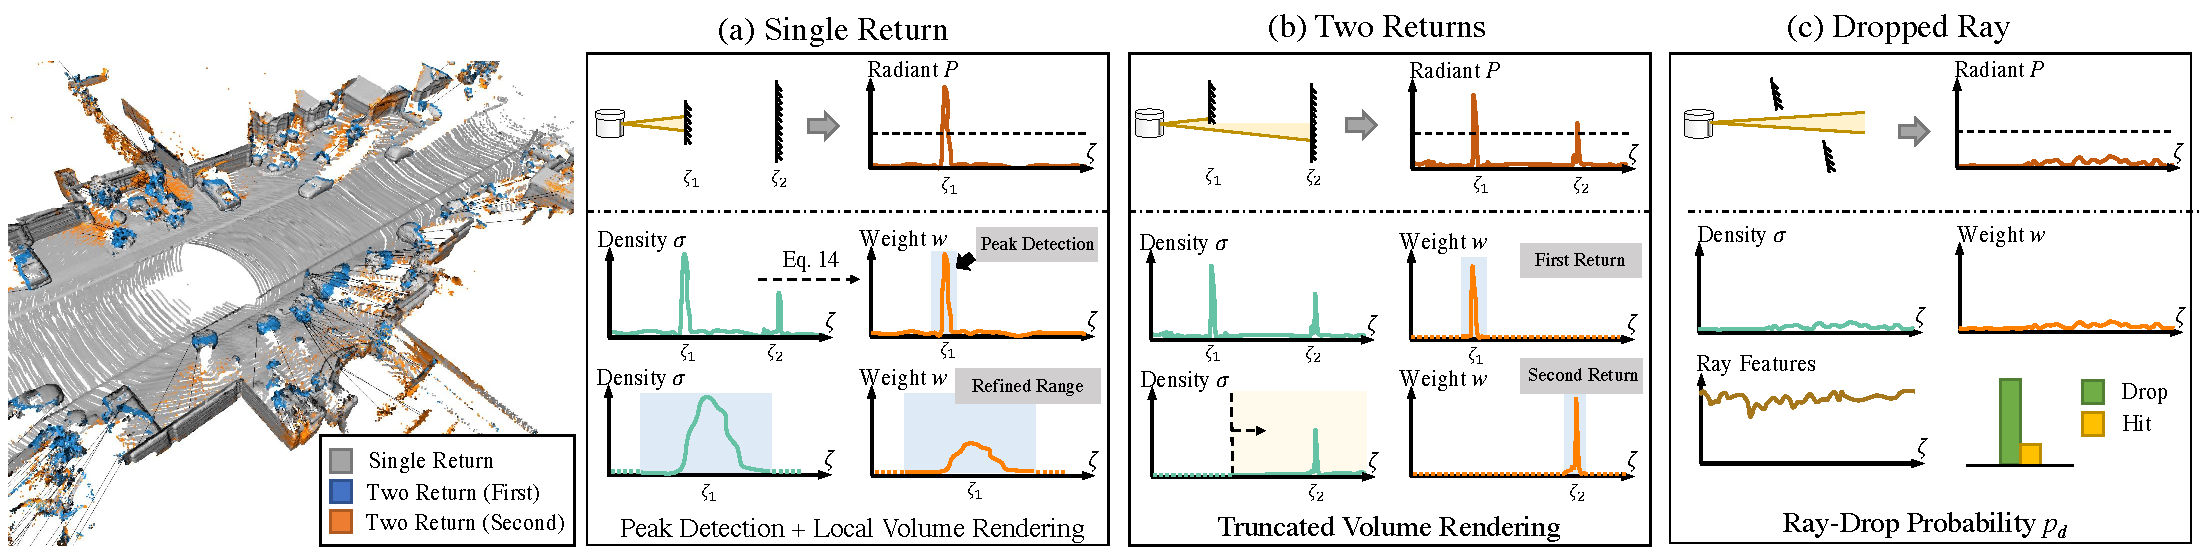
\includegraphics[width=1.0\columnwidth]{content/main/images/overview.pdf}
\caption{Left: real LiDAR scan demonstrating key LiDAR return properties: a \textcolor{mygray}{single return} and two returns (first return shown in \textcolor{myblue}{blue} and second return in \textcolor{myorange}{orange}). Right: NFL models the waveform and accurately reproduces these properties. (a) Top: the LiDAR energy is fully scattered by the first surface. Bottom: NFL estimates range via peak detection on the computed weights $w$ followed by volume rendering based range refinement. (b) Top: secondary returns resulting from a beam hitting two surfaces. Bottom: NFL employs beam divergence and a truncated volume rendering to estimate the second return. (c) Top: beams that do not hit a surface do not return detectable signal. Bottom: NFL utilizes geometric and semantic features to predict the ray drop probability. Refer to section \ref{sec:render_lidar} for more details. }
\label{fig:overview}
\end{figure}

